%\documentclass{neu_handout}
\documentclass[a4paper, 10pt]{article}

\usepackage{url}
\usepackage{amssymb}
\usepackage{hyperref}
\usepackage{enumitem}
\usepackage{graphicx}
\usepackage{subfig}
\usepackage{caption}

\usepackage{floatrow}


\usepackage{comment}  
\usepackage{fullpage} % changes the margin
\usepackage[margin=0.45in]{geometry}
\pagenumbering{gobble}          
\usepackage{hyperref}
\pagenumbering{arabic}    

\begin{document}


\title{DS5230 Project Update 1 : Pattern Recognition in Accidents in the UK}


\author{
  Sahasrabhojanee, Adwait\ \\     \texttt{sahasrabhojanee.a@husky.neu.edu}
  \and
  Sreekumar, Sreejith\  \\ \texttt{sreekumar.s@husky.neu.edu}
  \and
  Yu, Xue \\  \texttt{yu.xue1@husky.neu.edu}
  \and
  Li, Xuexian  \\ \texttt{li.xuex@husky.neu.edu}
}
\maketitle
\section{Introduction}
The Department of Transport in the United Kingdom has extensively recorded all the road accidents over the years. Their records provide a comprehensive dataset to
explore the patterns in road accidents and identify factors that add to their causality. \\
  As an initial study of the dataset, we explore noticeable patterns using statistical methods and exploratory data analysis. 

\section{Exploring accidents the UK region for trends and patterns }

\subsection{Spatial Study}  
The dataset comprises of accidents from England, Scotland and Wales. Making use of GPS data in the records, we isolated the top 200 cities/ suburbs where most number of
accidents have happened and geo-tagged them. \\

\begin{figure}[H]
    \begin{center}
      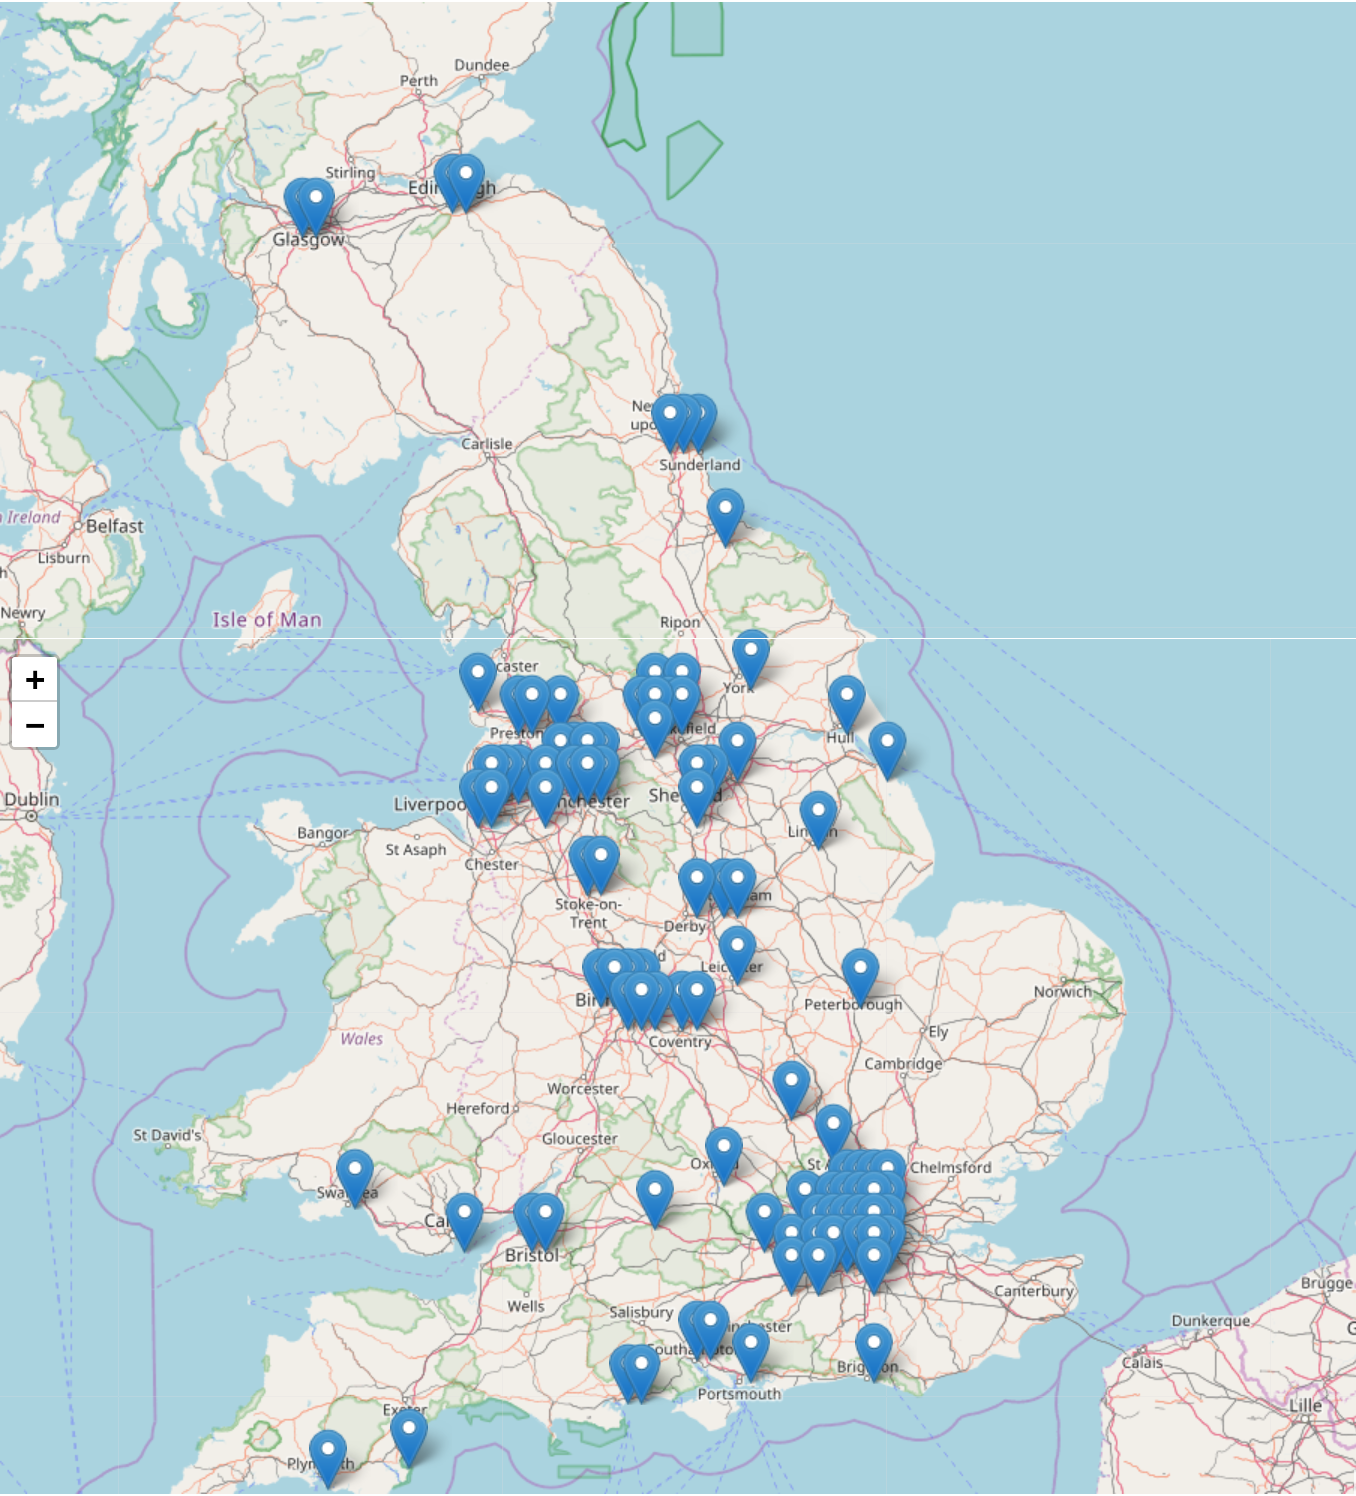
\includegraphics[width=105cm,height=9cm, scale=0.01,keepaspectratio]{map.png}
      \caption{Top 200 geographical locations where most accidents occur}
    \end{center}
\end{figure}

    Over the years from 2009-2014, the cities which stayed top 13 in the number of accident casualties are London, Birmingham, Kirklees, Liverpool, Leeds, City of Edinburgh, Wakefield, Rushcliffe, Sunderland, North East Derbyshire, Elmbridge, East Lindsey, and Manchester. As, we can see, there is a high concentration of pins around these areas. Unsurprisingly, these are the most populated cities in the UK[1]. \\

 We plotted a heat map showing the frequency of vehicles in different counties in the UK. The locations with high concentration of vehicles are more or less the same as the ones where the accidents are the highest. \\

 \begin{figure}[H]
   \begin{center}
     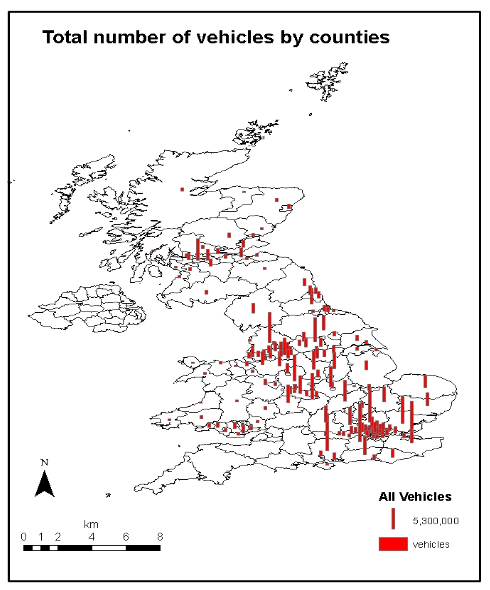
\includegraphics[width=70cm,height=6cm, scale=0.4,keepaspectratio]{vehicles-by-county.png}
     \caption{Total number of vehicles in various counties of U.K.(2014)}
    \end{center}
  \end{figure}

\subsection{Summary Statistics}
  Looking at the summary statistics of the records, we have: \\

\begin {table}[H]
 \caption {Summary Statistics}
    \begin{center}
 \begin{tabular}{c c c c c} 
  \hline
 Feature & Mean & Standard Deviation & Median & Mode \\ 
 \hline
 Police Force & 29.59 & 25.49 & 23 & 1  \\ 
 
 Number of Vehicles & 1.83 & 0.71 & 2 & 2 \\
 
 Number of Casualties & 1.34 & 0.82 & 1 & 1 \\

 Speed Limit & 38.52 & 13.9 & 30 & 30 \\
 \hline
\end{tabular}
  \end{center}
\end {table}

  It is seen that most accidents involve either two vehicles, or a single vehicle.. Mostly, 1 casualty occurs in an accident. \\

    The dataset groups the severity of the accidents in levels 1-3. However, it is not mentioned which is more severe on this scale. Since understanding this is critical to our analysis, we mapped the proportion of accidents in each severity level with the police force and the number of casualties. \\
\newline

\begin{figure} [H]
   \begin{center}
   \caption{Effect of Casualties and Police Force on Severity}
     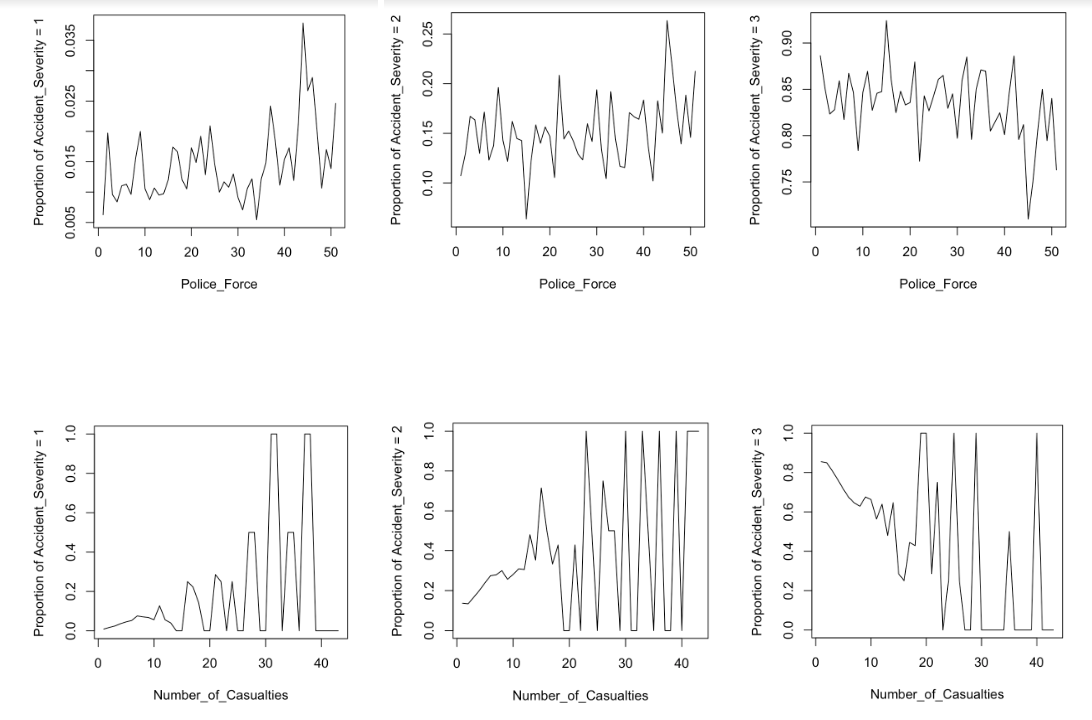
\includegraphics[width=70cm,height=7cm, scale=0.6,keepaspectratio]{severity-analysis.png}
   \end{center}
\end{figure}

As the number of casualties and the police force increases, the probability of the accident being assigned a severity of 1 increases, and the probability of being assigned a severity of 3 decreases. The probability of being assigned a severity of 2 increases sharply at first, but then slows down. This shows that a severity of 1 is the most severe, and a severity of 3 is the least severe. \\

 \subsection{Trends}
   
   \textbf{Trend in frequency of accidents over the years:}

\begin{figure}[H]
   \begin{center}
   \caption{Accidents by Year}
     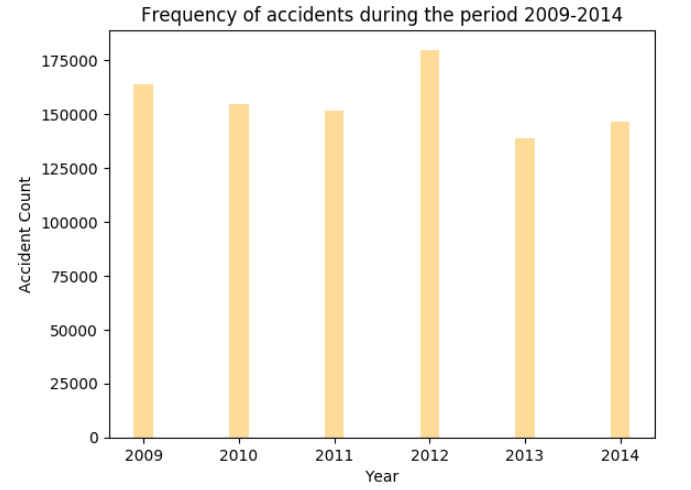
\includegraphics[width=20cm,height=5cm, scale=0.8,keepaspectratio]{counts.png}
   \end{center}
\end{figure}

   As seen in the bar plot, the accidents seem to have very slight variations, gradually decreasing trend mostly, over the years with an exception in 2012 when the number of accidents
   shot up over 175000. However, we don't know why this abrupt increase has happened yet. \\

   The variation in the number of accidents over different hours of the day indicates that most of the accidents occur between 3:00pm to 6:00pm and between 8:00 pm to 9:00 pm.
   This observation seems natural since these are the times when people are traveling to or returning from work.
   
\begin{figure}[H]
   \begin{center}
   \caption{Accidents by Hour}
     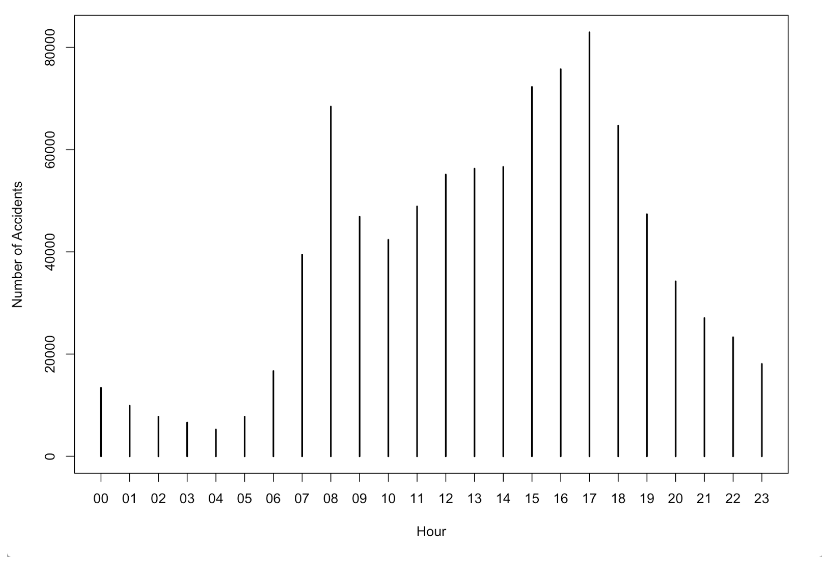
\includegraphics[width=10cm,height=6cm, scale=0.8,keepaspectratio]{hour-study.png}
   \end{center}
\end{figure}

\textbf{Seasonal frequency of road accidents:}

\begin {table}[H]
 \caption {Seasonal frequencies of Road accidents under various road conditions} \label{tab:title} 
    \begin{center}
 \begin{tabular}{l l l l l l l l l l l l l  } 
  \hline
 & Jan & Feb & Mar & Apr & May & Jun & Jul & Aug & Sep & Oct & Nov & Dec \\ 
 \hline
Fine with high winds&11.09&9.33&9.51&5.07&8.20&4.13&2.88&3.17&8.95&9.56&16.97&11.13\\
Fine without high winds&7.09&6.95&8.92&8.38&9.20&8.98&9.21&8.63&9.23&8.92&8.04&6.46\\
Fog or mist&15.50&10.12&12.96&2.84&1.38&2.33&1.11&1.24&3.44&9.93&18.74&20.42\\
Other&19.34&12.36&4.65&3.21&3.16&3.05&3.99&3.84&3.78&7.32&12.64&22.68\\
Raining with high winds&10.00&4.75&4.46&4.83&3.95&5.05&3.53&3.67&8.44&9.81&24.58&16.95\\
Raining without high winds&7.16&6.33&4.83&6.08&6.05&7.95&9.46&8.23&7.79&11.94&13.47&10.72\\
Snowing with high winds&19.41&26.06&18.51&3.23&0.54&0.00&0.18&0.18&1.08&0.99&4.22&25.61\\
Snowing without high winds&26.84&28.70&4.77&0.90&0.23&0.25&0.12&0.08&0.20&0.56&7.34&30.01\\
Unknown&10.09&8.61&7.73&7.04&7.96&7.27&7.25&6.77&7.74&9.20&10.70&9.64\\
 \hline
\end{tabular}
  \end{center}
\end {table}

   The analysis shows that 30.1\%, 26.84\% and 28.70\% of all accidents in snowy weather occurs in December, January and February respectively. The numbers are quite high for environments with
   fog or mist, as well as snow with high winds during these months. Maybe, taking more precautions and safety measures for the weather can bring down accidents during these months. \\

   \textbf{Trend in accident frequency with lighting conditions:}

\begin{figure}   [H]
   \begin{center}
   \caption{Yearly grouping of accidents by lighting conditions}
     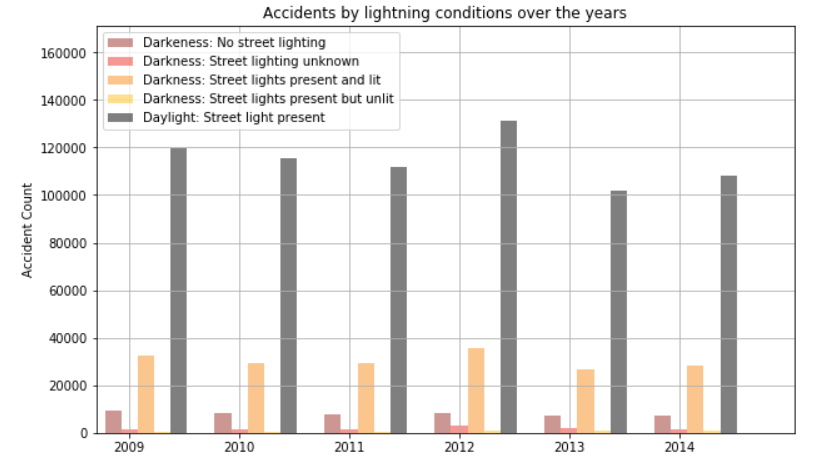
\includegraphics[width=70cm,height=7cm, scale=0.2,keepaspectratio]{lighting-study.png}
   \end{center}
\end{figure}

   The yearly trend for accident correlation with lighting conditions hasn't shifted much over the years. As we can see, most of the accidents occur during the daylight. The number of accidents that happen during night time on roads with street light are very less compared to this. \\
   Probably, most accidents didn't occur because of insufficient lighting. In addition, the chances that lights aren't lit if they were present are highly unlikely - this could be the reason why the fourth bar is short for every year. \\

   \textbf{Trend in accident frequency with weather conditions:}
\begin{figure}[H]
   \begin{center}
   \caption{Yearly grouping of accidents by weather conditions}
     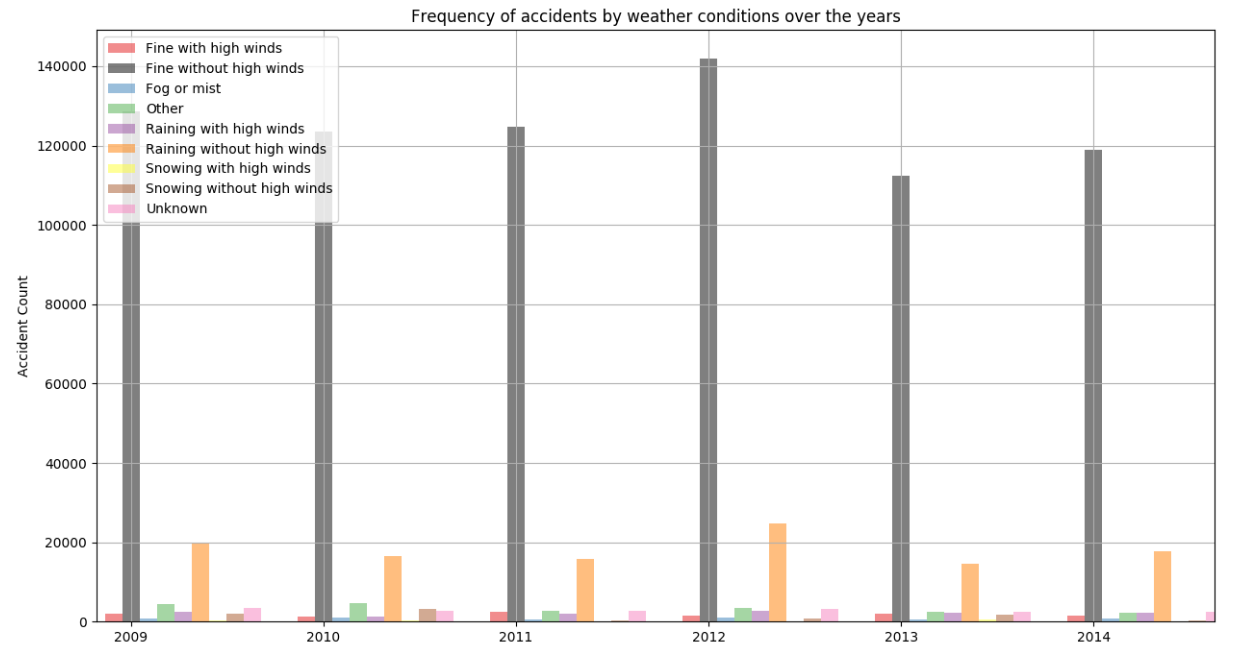
\includegraphics[width=70cm,height=7cm, scale=0.2,keepaspectratio]{weather-study.png}
   \end{center}
\end{figure}

   After analyzing the trend in the frequency of accidents with weather conditions during the period 2009-2014, we realized that most of the accidents happen during fine weather without any wind or storm.
 Although some accidents are weather prone as discussed before, it definitely isn't the main cause of accidents. \\
   
 \section{Outliers}
 \begin{itemize}
 \item For 11 accidents, the number of casualties was over 10, but no police officer attended the scene of the accident.
 \item There are 23 accidents in the dataset for which the recorded weather is snowy, but the month is May.
 \item There is 1 accident which involved 67 vehicles.  
 \end{itemize}
 
Some of these outliers are probably cases of data being recorded incorrectly, but some actually do make sense. For example, residents of Princetown and Rhayader in the UK woke up to a blizzard and 2 inches of snow in May 2013[2]. The weather can be really fickle!

\section{Next Steps}
Our main objective for this project is to use clustering for dimensionality reduction and for segmentation.

\subsection{Dimensionality Reduction}

Our data has over 900,000 rows and 33 variables, so working on it probably cause a substantial amount of downtime; this makes dimensionality reduction crucial to using this data.

\begin{itemize}
    \item We will first try creating new features by combining existing features and use those instead of the original features. For example, our analysis has shown that the weather conditions at the time of the accident are dependent on the month of the year; we could combine these variables in some way. 
    \item Next, we propose a method of checking if a categorical variable is redundant/highly dependent on other variables: We will hold out one categorical variable, and cluster the data using the rest of the variables. If the clusters formed approximately match the categories of the held-out variable, that might be an indication that the held-out column is not independent of the other variables.
    \item In the end we will apply principal component analysis to the numeric variables for further dimensionality reduction.
\end{itemize}

\subsection{Segmentation}
We will then use the data and use clustering to categorizing the accident into groups, to help better understand the similarity between certain accidents, and to check whether a large number of accidents can be avoided by taking only a few actions. We will probably use DBSCAN, because of its ability to exclude outliers, of which we have many.

   
\section{References}
 [1] \url{http://www.citymayors.com/gratis/uk\_topcities.html}
 \newline
 [2] \href{http://www.dailymail.co.uk/news/article-2324803/UK-weather-Its-middle-May-Two-inches-snow-months-rainfall-day-65mph-winds-hit-Britain.html} {Two inches of snow in May - dailymail.co.uk}
\end{document}

%%% Local Variables:
%%% mode: latex
%%% TeX-master: t
%%% End:
